\chapter{炎症}

本章主要介绍炎症局部的基本病理变化、急性炎症、慢性炎症、炎症的临床表现和结局。要求掌握炎症的概念,炎症局部的基本病变(变质、渗出和增生),急性炎症渗出性病变的反应过程包括血管反应、液体渗出和细胞渗出,液体渗出和白细胞对机体的防御作用,炎症介质的分类和主要作用,急性炎症的形态学类型及病变特点,慢性炎症的分类及病变特点;熟悉炎症的局部表现和全身反应,炎症的结局。

\section{概述}

\subsection{炎症的概念}

炎症(inflammation)是一种极常见又十分重要的病理过程,如疖、阑尾炎、肝炎、肺炎、肾炎、外伤感染等。当活组织被各种致病因子损伤时,损伤区域及周围组织发生以血管反应为中心的一系列变化,以便消除和局限病原因子,清除和吸收坏死的组织和细胞,随后过渡到修复,机体这种复杂的、以防御为主的反应称为炎症。炎症始于损伤又以修复告终,故损伤、炎症、修复三个病理过程是连续的有时相伴交叠进行,没有严格界限。

炎症的本质不是疾病,而是致炎因子引起的机体防御反应,是生物进化过程中获得并不断完善的抗病能力。炎症过程既保留了单细胞包围吞噬异物的自卫方式(白细胞具有此功能),又表现出由血管、神经、体液及白细胞共同参与的各种复杂的局部反应。当损伤因子刺激强烈、组织损伤严重时,常出现程度不等的全身反应。然而炎症不总是有益于机体,有时存在潜在的危害性,如过分剧烈的变态反应性炎症危及病人生命,心包、胸膜、肝、肾、脑和脑膜的重度炎症均可造成严重后果。正确认识炎症的发生、发展规律,对于防治炎症性疾病具有重要的意义。

\subsection{炎症形成的原因}

凡能引起机体组织和细胞损伤而诱发炎症的因素,统称为致炎因子。致炎因子种类繁多,一般可归纳为以下几类:

{1. 生物性因子}
 如细菌、病毒、立克次体、真菌、螺旋体、寄生虫等。这是一组最常见、也是最重要的致炎因子,它们引起的炎症称为感染(infection)。若感染病原体数量多、机体抵抗力低下,病原生物不仅引起局部的损伤,而且能在人体内繁殖、扩散。它们引起炎症的机制各不相同。例如,细菌主要通过内、外毒素作用;病毒则在机体细胞内生长并破坏细胞的正常代谢,导致细胞死亡引起炎症;也可因病原体通过其抗原诱发免疫反应,造成组织、细胞的损伤而发生炎症。

{2. 理化因子}
 物理性损伤,如高温、低温、放射线、激光、微波以及切割伤、挤压伤等。化学性损伤,如强酸、强碱、引起组织细胞损伤的药物,以及在病理条件下堆积于体内的代谢产物如尿酸、尿素等。

{3. 组织坏死}
 缺血或缺氧等原因可引起组织坏死,坏死组织是潜在的致炎因子。在新鲜梗死灶边缘出现的充血出血带和炎症细胞浸润都是炎症的表现。

{4. 变态反应}
 各型变态反应都可造成组织细胞损伤而引起变态反应性炎症,例如链球菌感染后肾小球肾炎。某些自身免疫性疾病也表现为炎症,例如结节性多动脉炎、溃疡性结肠炎等。

上述致炎因子是引起炎症的重要条件,但是否诱发炎症和引起炎症的程度如何,还取决于机体的抵抗力、免疫力、耐受性、组织特性等内在因素。例如,尽管新生儿神经系统尚未发育完善,但由于从母体获得了一定的抗体,所以新生儿对麻疹病毒和白喉杆菌有免疫作用,不易感染麻疹和白喉。先天性或后天性免疫缺陷患者,易发生正常人不易发生的某些细菌、真菌或寄生虫的机会感染。由此可见,机体的内在因素在炎症发生、发展中同样起了重要作用。

\section{炎症的基本病理变化}

炎症的基本病理变化包括变质(alteration)、渗出(exudation)和增生(proliferation)。在同一病变部位,这三者常按一定次序发生、发展,但往往有重叠,或以某种病变为主,有时也可互相转化。

\subsection{变质}

炎症局部组织发生的各种变性和坏死,统称变质。变质主要是由致炎因子的直接作用和炎症过程中出现的局部血液循环障碍引起。此时,局部组织细胞的代谢、功能也出现不同程度的障碍。组织细胞变性、坏死后,细胞的溶酶体膜崩解,释出多量水解酶,如蛋白酶、脂酶和磷酸酯酶,可进一步引起周围组织细胞的变性、坏死。

{1. 形态变化}
 炎症局部实质细胞的变性,包括细胞水肿、脂肪变等,坏死包括凝固性坏死、液化性坏死和干酪性坏死。间质常表现为黏液样变性、纤维素样坏死等。

{2. 代谢变化}
 主要表现为分解代谢增强,耗氧量增加。但由于酶系统受损和局部血液循环障碍,因此局部氧化代谢降低,产生许多氧化不全产物,如乳酸、脂肪酸、酮体、氨基酸等,在局部组织堆积,最后碱贮备消耗殆尽,引起局部酸中毒。一般说来,局部酸中毒在炎症灶中心最明显,炎症愈急剧,酸中毒愈明显。局部酸中毒一方面不利于病原微生物的生长,另一方面又给中性粒细胞的活动带来不利影响。此外还可使小血管受损,血管壁通透性增高。组织和细胞的酸中毒,还可使溶酶体膜受损,释放出多种炎症介质。

\subsection{渗出}

炎症局部组织血管内的液体和细胞成分通过血管壁进入组织间质、体腔、黏膜表面和体表的过程,称为渗出。渗出的血浆和细胞成分称为渗出物或渗出液(exudate)。渗出液在组织间隙中积聚引起水肿。当渗出液积聚在胸腔、腹腔、关节腔等浆膜腔内,称为炎性积液。炎症是以防御为主的病理过程,其中抗体和白细胞是两种最主要的防御成分。通过血管反应,抗体和白细胞得以渗出,并在局部消除致炎因子和有害物质。因此,血管反应是炎症中最重要的抗损伤过程。急性炎症反应的特征是血管变化和渗出性改变。

\subsection{增生}

炎症时增生是指在致炎因子或组织崩解产物等刺激下,病灶内巨噬细胞、纤维母细胞、内皮细胞、上皮细胞等增生和分化。在炎症早期,增生反应较轻微,在炎症后期较为明显。但某些急性炎症,例如急性弥漫性毛细血管内增生性肾小球肾炎和伤寒,则以增生性反应为主。炎症初期,来自血液和局部组织增生的巨噬细胞,具有吞噬病原微生物和清除组织崩解产物的作用。在炎症后期,纤维母细胞和血管内皮细胞增生明显,形成胶原和新生毛细血管,与浸润的炎细胞共同构成肉芽组织。出现肉芽组织,标志着炎症向愈复方向发展。

综上所述,任何致炎因子引起的炎症都具有变质、渗出和增生三种基本病理变化,只是不同类型的炎症以其中某一种基本病变为主。正如红、绿、蓝三原色的不同组合方式可混合出所有的颜色,变质、渗出、增生三种基本病理变化不同的比例,并且三者之间互相影响和转化,构成了不同类型的炎症反应。一般说来,变质反映了组织的损伤过程,而渗出和增生则反映了机体的抗损伤过程。急性炎症或炎症的早期,往往渗出性和变质性病变较显著,而慢性炎症或炎症的后期,则增生性病变较突出。但在炎症发展过程中,变质可以促进渗出和增生,渗出又可以加重变质。过度的增生不仅达不到修复的目的,还可能使疾病长期不愈或导致不良后果。因此,既要积极预防炎症性疾病的发生和发展,又要运用病理学知识,正确认识和区别损伤与抗损伤反应及其转化规律,采取适当的医疗措施,增强机体的防御能力,消除致炎因子,减少组织损伤,促进病变愈复。

\section{急性炎症}

炎症依其病程经过分为两大类:急性炎症(acute
inflammation)和慢性炎症(chronic
inflammation)。急性炎症反应迅速,持续时间短,常常仅几天,一般不超过一个月,病变以渗出性病变为主,炎症细胞浸润以中性粒细胞为主。慢性炎症持续时间较长,为数月到数年,病变以增生性变化为主,炎症细胞浸润以淋巴细胞和单核细胞为主。

急性炎症的主要特点是以血管反应为中心的渗出性变化,导致血管内的抗体和白细胞等透过血管壁进入炎症反应部位,消灭病原体,稀释并中和毒素,为炎症修复创造良好的条件。急性炎症时渗出性病变的反应过程包括血管反应、液体渗出和细胞渗出。

\subsection{血管反应}

急性炎症过程中组织发生损伤后,很快发生血流动力学变化,即血流量和血管口径的改变。血流动力学变化的速率取决于损伤的严重程度。血流动力学变化按如下顺序发生:

{1. 细动脉短暂收缩}
 致炎因子作用于局部组织,细动脉反射性短暂痉挛,持续数秒到数分钟。

{2. 血管扩张、血流加速}
 细动脉短暂收缩后随即扩张,毛细血管前括约肌开放,小动脉间交通支开放,局部血流加快,血灌注量增多,形成动脉性充血。局部组织因而发红、温度升高、代谢增强,持续数分钟到几小时不等。血管扩张机制早期是由于轴突反射和血管运动神经兴奋,持久性扩张是由于炎症介质的作用。

{3. 血流速度减慢、血流停滞}
 由于炎症介质的作用,使血管壁通透性升高,血浆蛋白和液体在毛细血管静脉端和微静脉渗出,引起血液浓缩,黏滞性增加,导致血流缓慢,形成静脉淤血。同时,毛细血管及微静脉内的流体静压增高,以致大量血浆漏出,使局部组织水肿,血液的黏稠性更加增大。随血流速度减慢,红细胞聚集成团,边流消失,白细胞靠边和逸出。当血流几乎停止或只是晃动时称为淤滞(stasis),局部呈紫红色。严重时还可发生血栓形成或出血(图\ref{fig4-1})。

\begin{figure}[!htbp]
 \centering
 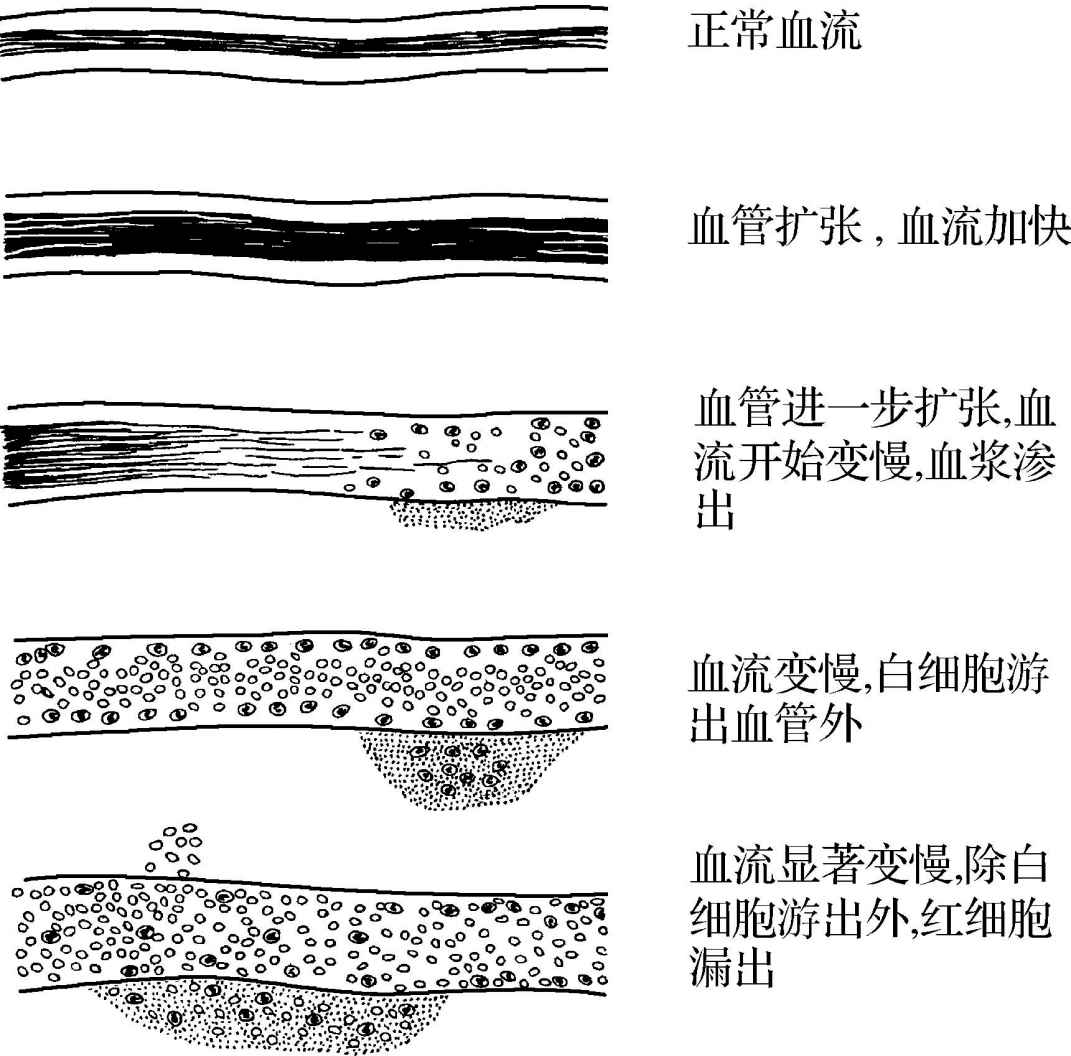
\includegraphics[width=0.5\textwidth]{./images/Image00050.jpg}
 \caption{急性炎症血管反应模式图}
 \label{fig4-1}
\end{figure} 

上述血管反应发展的速度与致炎因子性质和损伤的严重程度相关。极轻微的损伤仅引起血流加速,持续10~15分钟,迅速恢复正常,不出现渗出和血流减慢的改变。轻度损伤表现为持续血流加快数小时,血量增加,然后进展至血流缓慢,最后淤滞。重度损伤仅短暂的动脉性充血,血量增加,几分钟内就发生淤滞。此外,炎症局部的不同区域,血管反应也不一致,如烫伤中心区呈现淤滞时,周边区尚表现为血管扩张、血流量增加。

\subsection{液体渗出}

由于血管壁受损的程度不同,液体渗出的成分也有差别。血管壁受损轻微时,渗出液中仅含盐类和小分子白蛋白。当血管壁受损严重时,分子量较大的球蛋白甚至纤维蛋白也能渗出。

炎性渗出液与单纯因流体静压升高形成的漏出液不同,两者的区别见表\ref{tab4-1}。


    \begin{table}
        \centering
    \caption{渗出液与漏出液的鉴别}
    \label{tab4-1}
    \begin{tabular}{ccc}
    \toprule
    & 渗出液 & 漏出液 \\
    \midrule
    蛋白质 & >30g/L & <25g/L\\
    比重 & >1.018 & <1.018\\
    细胞数 & $>5\times 10^8/\text{L}$ &
    $<1\times 10^8/\text{L}$\\
    Rivalta试验 & 阳性 & 阴性\\
    凝固 & 能自凝 & 不能自凝\\
    透明度 & 混浊 & 澄清\\
    \bottomrule
    \end{tabular}
    \end{table}

液体渗出的原因和机制十分复杂,其中有些尚未完全阐明,主要归纳为三个方面,即血管壁通透性升高、毛细血管内流体静压增高和炎症区域内组织渗透压升高。一般而言,液体渗出是这三方面因素共同作用的结果。

{1. 血管壁通透性升高}
 这是液体渗出最主要的原因,主要发生于微静脉和静脉端毛细血管。正常的微循环,血管通透性主要依赖于内皮细胞的完整性。在炎症过程中,下列机制可引起血管通透性升高:

(1)内皮细胞收缩:内皮细胞收缩是由速发短暂反应和内皮细胞骨架重构两种机制引起。组织胺、缓激肽和其他炎症介质与内皮细胞受体结合以后,可迅速引起内皮细胞收缩,细胞间隙增宽。由于这些炎症介质的半寿期较短,仅15~30分钟,故这种反应被称为速发短暂反应。此反应累及微静脉,而细动脉和毛细血管不受累。抗组织胺药物能抑制此反应。内皮细胞收缩的另一个机制是内皮细胞骨架重构。

(2)直接内皮损伤:如严重烧伤和化脓性细菌感染等严重刺激可直接造成内皮细胞损伤,使之坏死和脱落,迅速出现血管壁通透性升高,并在高水平上持续几小时到几天,直至受损血管内形成血栓,此过程称为速发持续反应。微循环各级血管均可累及。

(3)迟发持续性渗漏:轻度和中度热损伤、X线和紫外线损伤以及某些细菌毒素引起的内皮细胞直接损伤或Ⅳ型变态反应等发生较晚,常在2~12小时之后,但可持续几小时到几天,称为迟发持续反应。此反应仅累及毛细血管和小静脉,其形成机制可能与内皮细胞凋亡或细胞因子作用有关。

(4)白细胞介导的内皮损伤:在炎症的早期,白细胞附壁并与内皮细胞黏附,引起白细胞激活,释放具有生物活性的氧自由基和蛋白水解酶,引起内皮细胞的损伤或脱落,使血管壁通透性增加。

(5)新生毛细血管壁的高通透性:在修复过程中所形成的新生毛细血管芽,其内皮细胞连接发育不成熟,使液体外渗和水肿。

{2. 微循环内流体静压升高}
 由于炎症区域内的细动脉和毛细血管扩张,静脉淤血、血流缓慢,使毛细血管内流体静压升高,血管内液体渗出增多。

{3. 组织渗透压升高}
 炎症时,组织变质,使局部组织中许多大分子物质分解为小分子物质,因而胶体渗透压升高;组织的分解代谢增强,钾离子、磷酸根离子及其他离子浓度升高,因而晶体渗透压也升高。这些均促进了液体的渗出。

液体的渗出对机体具有重要防御意义:①稀释和中和毒素,减轻毒素对局部的损伤作用。因为大量的渗出液能稀释毒素,带走炎症灶内的有害物质;②渗出液中有丰富的抗体和补体,有利于消灭病原微生物;③渗出的纤维素交织成网,可以阻止病原菌的扩散,并有利于白细胞发挥吞噬作用;④渗出物中的病原微生物和毒素随淋巴液被带到局部淋巴结,有利于细胞和体液免疫的产生。

但若渗出液过多,也可压迫周围的组织和器官,造成不良后果,例如心包或胸腔积液分别压迫心脏和肺脏,严重喉头水肿可引起窒息;纤维素渗出若不能被完全溶解吸收,则会发生机化,引起器官和组织的粘连,例如肺肉质变和缩窄性心包炎。

\subsection{白细胞的渗出和吞噬作用}

炎症过程中不仅有液体渗出,而且还有白细胞渗出。各种白细胞由血管内渗出到组织间隙的现象,称为炎细胞浸润(inflammatory
cell
infiltration)。白细胞,特别是中性粒细胞和巨噬细胞,能吞噬病原微生物、异物和坏死组织碎片。渗出的白细胞也称为炎细胞(inflammatory
cell)。白细胞渗出与液体渗出的机制不同,是主动过程,包括靠边、附壁、游出、趋化和吞噬。

{1. 白细胞靠边、附壁和黏着}
 炎症时,随着血流速度减慢,轴流变宽,白细胞进入边流,向管壁靠拢,称白细胞靠边(leukocytic
margination)。白细胞与内皮细胞相接触,初时尚可缓慢滚动,以后则与内皮细胞附着,形成白细胞的附壁黏着。

虽然多种因素影响着内皮细胞与白细胞的附壁黏着,诸如内皮细胞和白细胞表面负电荷被中和而相互排斥力下降,二价阳离子桥接内皮细胞与白细胞而促进黏着等,但目前认为这种黏着是内皮细胞和白细胞表面的黏附分子介导的,包括免疫球蛋白超家族分子和整合蛋白类分子。炎症可诱导内皮细胞和炎症细胞表达新的黏附分子,增加黏附分子的数目和增强彼此的亲和性。

{2. 白细胞游出}
 白细胞通过血管壁进入周围组织的过程,称为白细胞的游出(emigration)。白细胞附壁后以阿米巴样方式运动,先伸出伪足插入内皮细胞间连接,穿过变宽的连接间隙,通过变形运动,整个细胞游出到内皮细胞与基底膜之间,最后穿过基底膜到达血管外。这种游出过程依靠白细胞胞浆反复从凝胶状态转变为溶胶状态而完成。当细胞一部分变为溶胶状态就形成伪足,向前伸展,接着这部分胞浆转化为凝胶状态,胞体收缩并同时向前移动,在游出过程中,内皮细胞收缩使细胞间隙增宽。还有学者发现炎症时内皮细胞胞突伸长将白细胞包围,以协助白细胞游出,同时限制血浆渗出(图\ref{fig4-2})。中性粒细胞游出血管壁需2~8分钟。

\begin{figure}[!htbp]
 \centering
 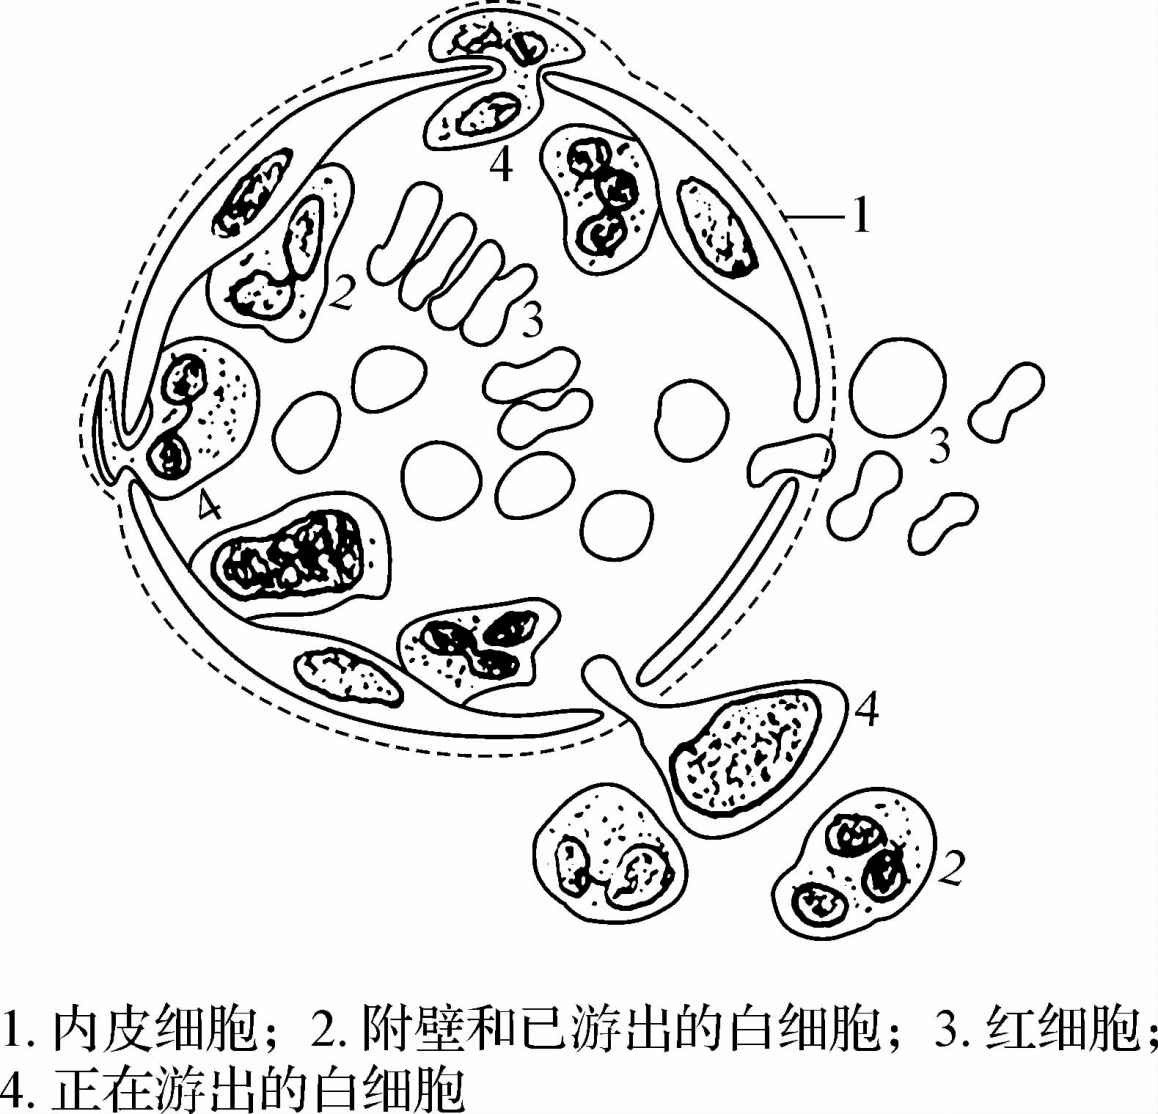
\includegraphics[scale=1.2]{./images/Image00052.jpg}
 \caption{白细胞游出示意图}
 \label{fig4-2}
  \end{figure} 

游出的白细胞最初围绕血管周围,随后沿组织间隙以15~20
μm/min的速度作阿米巴样定向游走,向炎症灶中心区聚集。白细胞一旦游出血管就不再返回血流。有时红细胞也可随白细胞透出,这是由于血管内流体静压将它从白细胞游出的微小缺口挤出。内皮受损严重时,红细胞会大量漏出,构成出血性炎症。

急性炎症时,一般中性粒细胞首先游出,单核细胞和淋巴细胞稍后游出,但伤寒以单核细胞游出为主。病毒感染或免疫反应时,以淋巴细胞游出和积聚为显著。一些过敏反应中则以嗜酸性粒细胞浸润为主。研究结果表明,在急性炎症的最初几日,中性粒细胞的游出最多。以后,单核细胞逐渐增多,超过中性粒细胞,且持续时间亦长。这可能与中性粒细胞的溶酶体酶能趋化单核细胞有关。中性粒细胞游出血管后仅存活24~48小时,在酸性环境中容易死亡。而巨噬细胞寿命长,且能在组织中进行分裂。值得注意的是,白细胞是主动游出,故与血管壁通透性升高不成平行关系。

白细胞血管内皮细胞间黏附分子、血管内皮细胞间黏附分子在白细胞游出中具有重要作用,此外,还与炎区组织中产生的一些具有趋化作用的化学物质有关。

{3. 趋化作用}
 白细胞从血管内游出到血管周围后,朝化学刺激物所在部位作定向游走,称为趋化作用(chemotaxis)。能吸引白细胞作趋化游走的化学物质称为趋化因子。

白细胞的趋化因子有多种,如IgG的衍化物白细胞游出素(leukoegresin),可特异地趋化中性粒细胞;中性粒细胞释出的阳离子蛋白和淋巴细胞产生的淋巴因子对单核细胞有趋化作用;肥大细胞释放的嗜酸性粒细胞趋化因子(ECF-A)对嗜酸性粒细胞有很强的趋化作用;补体片段,特别是C{5a}
对中性粒细胞、单核细胞、嗜酸性粒细胞均有趋化作用。此外,纤维素、胶原、组织崩解产物、细菌毒素及其代谢产物、病毒感染的细胞等,多通过激活补体而发挥趋化作用。

趋化作用是个十分复杂的生物学现象,确切机制尚未阐明。近年研究表明,趋化因子是通过靶细胞表面的特异性受体而发挥作用的。

{4. 吞噬作用}
 白细胞在炎症灶内对病原体和崩解的组织碎片进行识别、吞噬、杀灭和分解的过程,称为吞噬作用(phagocytosis)。人体的吞噬细胞主要有两种,即中性粒细胞(小吞噬细胞)和巨噬细胞(大吞噬细胞)。其他白细胞的吞噬能力均很弱。吞噬过程包括识别和黏着、吞入、杀灭和降解三个阶段(图\ref{fig4-3})。

\begin{figure}[!htbp]
 \centering
 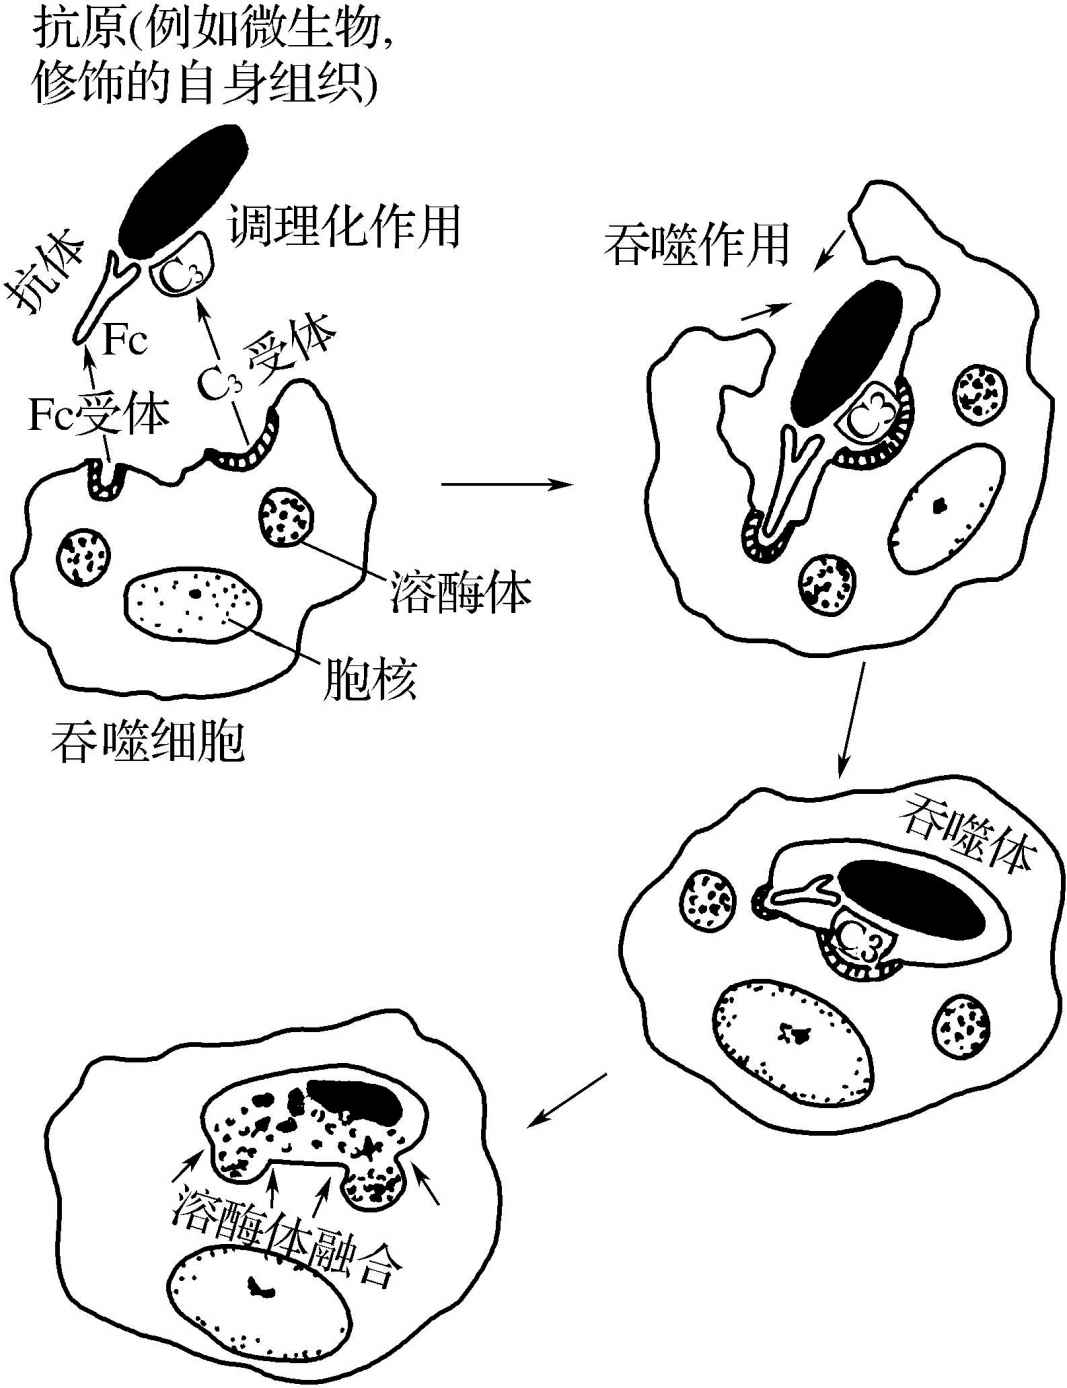
\includegraphics[scale=1.2]{./images/Image00053.jpg}
 \caption{吞噬过程示意图 \\ {\small 吞噬细胞的识别、吞噬和降解}}
 \label{fig4-3}
  \end{figure} 



(1)识别和黏着:血清中存在着调理素(opsonin),所谓调理素是指一类能增强吞噬细胞吞噬功能的蛋白质,包括IgG的Fc段、补体C{3b}
等。它们覆盖在病原体的表面,可被吞噬细胞膜上的特异性免疫球蛋白Fc受体(FcγR)、补体受体(CR{1}
、CR{2} 、CR{3} )识别。

(2)吞入:识别附着后,吞噬细胞即形成伪足,并且伸长、包绕、融合,将病原体包围吞噬,形成吞噬体(phagosome)。

(3)杀灭和降解:吞噬体与溶酶体融合,形成吞噬溶酶体(phagolysosome),病原体在溶酶体水解酶的作用下被杀灭和降解。含有已被降解和消化了的异物残渣的溶酶体称为残体。

通过吞噬细胞的杀灭作用,大多数病原微生物被杀灭。但有些细菌在白细胞内处于静止状态,依然具有生命力和繁殖力,如结核杆菌。一旦机体抵抗力下降,这些病原体又能繁殖,并可随吞噬细胞的游走而在体内播散。生活在吞噬细胞内的细菌难以受到抗生素和机体防御机制的影响,故不易被消灭。

杀灭和降解病原体的机制包括依赖氧的杀伤机制和不依赖氧的杀伤机制两种。

白细胞在局部还具有免疫作用。发挥免疫作用的细胞主要为单核细胞、淋巴细胞和浆细胞。抗原进入机体后,巨噬细胞将其吞噬处理,再把抗原呈递给T和B细胞,免疫活化的淋巴细胞分别产生淋巴因子或抗体,发挥杀伤病原微生物的作用。

白细胞在吞噬过程中不仅可向吞噬溶酶体内释放产物,而且还可将产物释放到细胞外间质中。中性粒细胞释放的产物包括溶酶体酶、活性氧自由基、前列腺素和白细胞三烯,这些产物可引起内皮细胞和组织损伤,加重最初致炎因子的损伤作用。由此可见,如能控制白细胞一定程度的渗出才是更有益的。

\subsection{炎细胞的种类}

常见的炎细胞(图\ref{fig4-4})有以下几种:

\begin{figure}[!htbp]
 \centering
 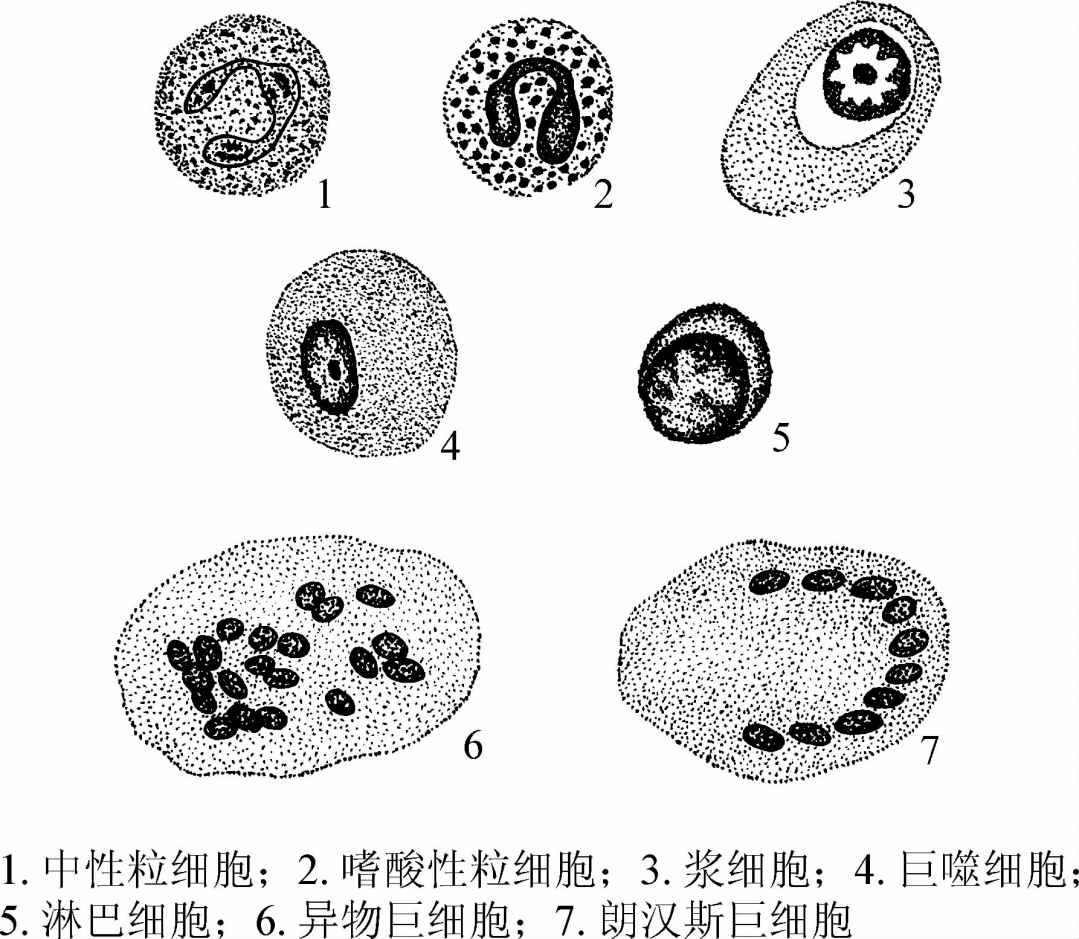
\includegraphics[width=0.5\textwidth]{./images/Image00054.jpg}
 \caption{几种常见的炎细胞}
 \label{fig4-4}
  \end{figure} 

{1. 中性粒细胞}
 是化脓性炎或急性炎症中最常见的炎细胞,亦可见于慢性炎症急性发作时。

{2. 单核细胞及巨噬细胞}
 血液中的单核细胞进入组织后则转化为巨噬细胞,它具有很强的吞噬功能。常见于急性炎症后期或慢性炎症。

{3. 淋巴细胞和浆细胞}
 多见于慢性炎症、病毒所致炎症以及与免疫反应有关的炎症。

{4. 嗜酸性粒细胞}
 多见于各种慢性炎症,尤其是寄生虫引起的炎症和I型变态反应性炎症。

{知识链接}

中性粒细胞在局部抗感染中发挥十分重要的作用。当机体遭受病原微生物,特别是化脓性细菌感染时,中性粒细胞即发挥其防御功能。近年研究表明,当病原微生物引起感染时,中性粒细胞可释放中性粒细胞胞外诱捕网(neutrophil
extracellular traps
NETs),网罗、杀伤病原体从而参与机体自身免疫应答。NETs由DNA纤维网、组蛋白、髓过氧化物酶、中性粒细胞弹性蛋白酶、组织蛋白酶和抗菌肽等构成。

中性粒细胞胞外诱捕网也是把双刃剑,在局部感染期间由于能捕捉和杀灭病原体对机体是有利的,但在系统性感染时由于对肺泡上皮细胞的毒性可造成急性肺损伤,以及对内皮细胞和凝血系统的影响可诱发DIC,都可能增加脓毒症患者的病死率。NETs也参与了系统性红斑狼疮、类风湿关节炎、小血管炎等自身免疫性疾病的发生和发展,这些都是对机体不利的影响。

{5. 嗜碱性粒细胞和肥大细胞}  常见于变态反应性炎症。

\subsection{炎症介质}

炎症反应中除早期有神经介导作用外,都是通过化学介质发挥作用的,尤其是急性炎症时,局部反应的每个阶段都与化学介质的作用密切相关。炎症过程中参与介导炎症反应的化学因子称为炎症介质(inflammatory
mediator)。炎症介质有内源性和外源性两种,内源性炎症介质又可分为细胞释放的炎症介质和体液中产生的炎症介质两种。

{(一)细胞释放的炎症介质}

{1. 血管活性胺}
 包括组织胺和5-羟色胺。组织胺存在于肥大细胞、嗜碱性粒细胞和血小板中。组织胺可使细动脉和毛细血管扩张、微静脉内皮收缩,导致血管壁通透性增高。组织胺对嗜酸性粒细胞还有趋化作用。5-羟色胺在人类炎症中的作用不很明显。

{2. 花生四烯酸代谢产物}
 包括前列腺素和白细胞三烯两大类产物。体内几乎所有细胞都能合成前列腺素。前列腺素除了有强烈的扩血管作用及使血管壁通透性增高的作用外,还具有致热和致痛作用。白细胞三烯主要由白细胞和肥大细胞合成,具有强烈的增高血管壁通透性的作用(为组织胺的200~1
000倍),白细胞三烯中的B{4} 成分还具有白细胞趋化作用。

{知识链接}

一个多世纪以来,人们发现阿司匹林有较强的消炎、解热和镇痛作用,但具体机制并不明确。英国药理学家John
Robert
Vane揭开了这一谜团,因此他获得了1982年诺贝尔医学奖。原来花生四烯酸通过环氧化酶(cyclooxygenase
COX)合成前列腺素,后者作为重要的炎症介质,参与了多种炎症反应,可引起血管扩张、组织水肿、发热和疼痛。COX共有3种亚型,其中COX-2和COX-3参与炎症反应,而COX-1则对胃黏膜起保护作用。阿司匹林可同时抑制这三种COX,在消炎镇痛的同时却造成了胃黏膜的损伤,引起胃肠道反应、胃炎甚至胃溃疡。使用阿司匹林肠溶片,以及特异性COX-2抑制剂则可减轻这些副作用。

{3. 白细胞产物}
 主要为中性粒细胞、单核巨噬细胞释放的氧自由基和溶酶体酶成分。

(1)氧自由基:为吞噬细胞吞噬后的依赖氧杀菌机制产生。氧自由基可以与细胞膜上的脂质发生过氧化反应,破坏细胞膜的稳定性,除了杀菌作用以外也可导致细胞、组织的损伤(如内皮细胞的损伤可引起血管壁通透性增高)。氧自由基还可灭活一些抗蛋白酶类(如α{1}
-抗胰蛋白酶),导致炎症时细胞释放的蛋白酶活性过高,使周围正常组织遭到破坏,引起扩大的组织损伤。

(2)中性粒细胞溶酶体成分:包括酶与非酶两类成分,在中性粒细胞吞噬时外逸或中性粒细胞死亡时释放。酶类中的中性蛋白酶(包括弹力蛋白酶、胶原酶等)、酸性蛋白酶(包括组织蛋白酶A、B、C、D、E等)可介导细胞、组织的损伤。非酶类的阳离子蛋白能刺激肥大细胞,使其脱颗粒释放组织胺,直接或间接地引起血管扩张、通透性增高及趋化白细胞和杀菌作用,阳离子蛋白还具有致热源的作用,可引起机体发热。

{4. 细胞因子}
 主要由激活的淋巴细胞、单核巨噬细胞产生。细胞因子可调节其他炎症细胞的功能,特别是细胞免疫反应的发生和发展,在介导炎症反应中也有重要作用。在炎症中起重要作用的细胞因子有:

(1)白细胞介素(interleukin,IL)与肿瘤坏死因子(tumor necrotic
factor,TNF):IL-1和TNF可促进内皮细胞表达黏附分子,有利于白细胞游出过程中的黏附作用。两者都有致热源的作用,可引起机体发热。IL-1还有促进纤维母细胞、内皮细胞增生的作用。IL-8、TNF具有强烈的中性粒细胞趋化和激活作用(TNF还可促使溶酶体酶释放,引起组织损伤)。

(2)淋巴因子(lymphokine):如巨噬细胞游走抑制因子、活化因子、趋化因子(MIF、MAF、MCF),白细胞趋化因子、游走抑制因子(LCF、LIF)等。

{5. 血小板激活因子(platelet activating factor,PAF)}
 目前已知PAF来源于活化的嗜碱性粒细胞、肥大细胞、中性粒细胞、单核巨噬细胞、血管内皮细胞及血小板本身。PAF作用于血小板,使之激活、聚集,影响血流动力学改变;增加血管通透性,促使白细胞与内皮细胞黏着,以及影响趋化作用和促使白细胞脱颗粒;PAF还有刺激白细胞和其他细胞合成前列腺素和白细胞三烯的作用。

{6. 一氧化氮(NO)}
 主要是由内皮细胞、巨噬细胞和一些特定神经细胞在一氧化氮合酶(NOS)作用下生成的。NO参与炎症过程,主要是作用于血管平滑肌,使血管扩张;抑制血小板黏着和聚集、抑制肥大细胞引起的炎症反应;调节、控制白细胞向炎症灶的集中。细胞内大量NO可减少微生物复制,但也可造成组织细胞的损伤。

{7. 神经肽}
 如P物质,存在于肺和胃肠道的神经纤维,有传递疼痛信号、调节血压、刺激免疫细胞和内分泌细胞分泌的作用。P物质是增加血管通透性的强有力的介质。

{(二)体液源性的炎症介质}

血浆中存在相互关联的四大炎症介质系统。

{1. 激肽系统}
 激肽系统被激活后可产生一系列中间产物,其最终产物为缓激肽。缓激肽的作用主要为扩张细动脉、增强血管壁通透性(其作用强度相当于组织胺的800倍)和强烈的致痛作用。

{2. 补体系统}  与炎症有关的补体片段主要为C{3a} 、C{5a} 和C{567} 。C{3a}
、C{5a} 又称过敏毒素,能促使肥大细胞和血小板释放组织胺;C{5a} 、C{567}
对吞噬细胞有强烈的趋化作用;C{3b} 具有调理素作用,可增强吞噬作用。

{3. 凝血系统}
 在凝血系统激活过程中,凝血酶激活纤维蛋白原时产生酶解片段纤维蛋白和纤维蛋白多肽,后者可使血管壁通透性增高,并具有白细胞趋化作用。

{4. 纤溶系统}
 纤溶系统激活后产生的纤维蛋白降解产物也具有增高血管壁通透性和白细胞趋化作用。

{(三)炎症介质的作用特点}

综上所述,炎症介质具有如下一些共同特点:

1.
很多炎症介质通常是以其``前体''或``非活性''状态存在于体液或细胞之中,经多步骤的激活后才能发挥作用,其活性状态的半衰期往往较短,一旦释放或激活,即被迅速灭活破坏,从而维持动态平衡。

2. 炎症介质的释放可同时激活起反作用的拮抗物,起到负反馈调节作用。

3.
各种炎症介质的致炎效应不尽相同,某些炎症介质可表现为多种致炎效应,而不同的炎症介质也可表现出相同的致炎效应。

4.
不同的炎症介质系统之间有着密切的联系,如激肽、补体、凝血和纤溶系统的激活产物在炎症反应中是重要的炎症介质。组织损伤时激活的Ⅻ因子(hageman
factor)可启动上述四大系统的激活,各系统激活过程中的中间产物也可激活其他系统。

主要炎症介质的种类及其生物学作用归纳如表\ref{tab4-2}。

    \begin{longtable}{cc}
    \caption{炎症中的主要介质及其作用}
    \label{tab4-2}\\
    \toprule
    作用 & 主要炎症介质\\
    \midrule
    扩张血管 & 组胺、缓激肽、前列腺素、\ce{NO}\\
    增加血管壁通透性 & 组胺、缓激肽、\ce{C_{3a}}和\ce{C_{5a}}、白细胞三烯、PAF、P物质\\
    趋化作用 & 白细胞三烯、\ce{C_{5a}}、细菌产物、阳离子蛋白、化学因子\\
    发热 & IL-1、IL-2、TNF-α、前列腺素\\
    疼痛 & 前列腺素、缓激肽\\
    组织损伤 & 氧自由基、溶酶体酶、\ce{NO}\\
    \bottomrule
    \end{longtable}



\subsection{急性炎症的形态学类型}

炎症反应的发生发展过程复杂多样,由于致炎因子和组织防御反应的不同,急性炎症的形态学类型也有所差异。炎症包括变质、渗出和增生三种基本病理变化,因而根据不同的病理变化将急性炎症分为变质性炎、渗出性炎和增生性炎三种类型。

{(一)变质性炎}

变质性炎(alterative
inflammation)是以局部组织的变性和坏死为主要病变,常见于感染、中毒和变态反应,主要发生于肝、肾、心和脑等实质器官。例如急性病毒性肝炎,肝细胞可出现细胞水肿、溶解性坏死等病变;流行性乙型脑炎,神经细胞变性、坏死以及脑软化灶形成;阿米巴感染造成肝细胞大量坏死形成阿米巴脓肿。由于病变器官的实质细胞变性、坏死,变质性炎常导致器官的功能障碍。

{(二)渗出性炎}

渗出性炎(exudative
inflammation)在急性炎症中最为常见,病变以渗出性改变为主,病灶内形成大量渗出物。由于致炎因子和机体反应的不同,渗出物的成分也有所不同。根据渗出物的主要成分,通常将渗出性炎分为浆液性炎、纤维素性炎、化脓性炎和出血性炎等几种类型。

{1. 浆液性炎}  浆液性炎(serous
inflammation)以浆液渗出为其特征,浆液性渗出物以血浆成分为主,也可由浆膜的间皮细胞分泌,含有3%~5%的小分子蛋白质(主要是白蛋白)、少量白细胞和纤维素。浆液性炎主要发生于浆膜、黏膜和疏松结缔组织等处,如感冒初期的鼻炎、皮肤Ⅱ度烧伤所形成水泡(图\ref{fig4-5})、风湿性关节炎的关节腔积液等都是属于浆液性炎的表现。

\begin{figure}[!htbp]
 \centering
 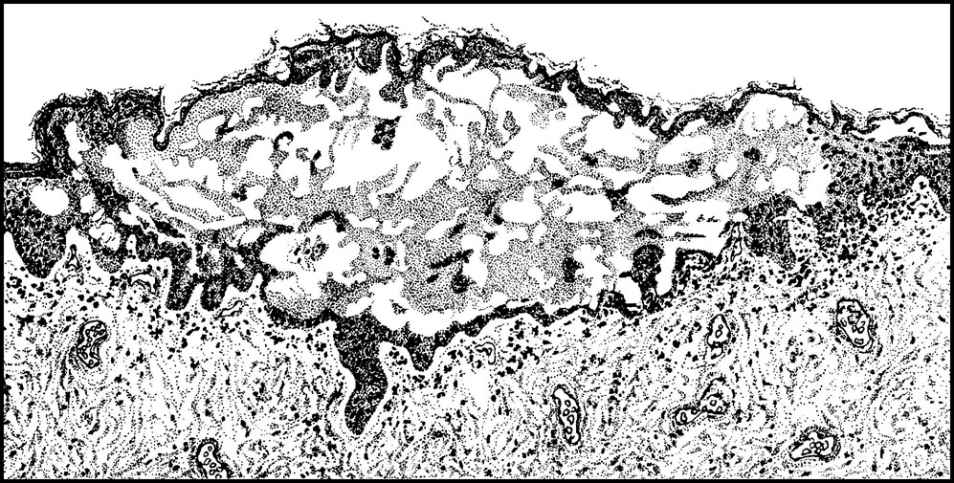
\includegraphics{./images/Image00056.jpg}
 \caption{皮肤浆液性炎(疱疹)\\ {\small 表皮层内有一大水泡形成,其中含多量浆液}}
 \label{fig4-5}
  \end{figure} 

浆液性炎组织损伤较小,病因消除后渗出的成分易于吸收消散,由于组织没有明显的破坏,因此愈后一般不留痕迹。炎症过程中如果渗出过多则可导致严重后果,如心包腔内过多的浆液性渗出可影响心肺的功能,喉头浆液性炎造成的喉头水肿可引起窒息。

{2. 纤维素性炎}  纤维素性炎(fibrinous
inflammation)是以大量纤维蛋白原渗出为主,并在炎症灶内形成纤维素为特征的炎症。此时血管壁的损伤较重,通透性较浆液性炎时增高更为明显,以至于大分子的纤维蛋白原大量渗出。

纤维素性炎常由细菌毒素(如白喉杆菌、痢疾杆菌、肺炎球菌毒素等)或有毒物质(如尿毒症时的尿素、汞中毒等)引起,常发生于黏膜、浆膜和肺。镜下(HE染色)观:纤维素为红染、网片状或细丝状物,夹杂有一定量的中性粒细胞。发生于黏膜的纤维素性炎(如白喉、细菌性痢疾)纤维素、白细胞和坏死的黏膜上皮常混杂在一起,形成灰白色的膜状物,覆盖在黏膜的表面,称为``假膜''(或伪膜)。因此,黏膜的纤维素性炎又称为``假膜性炎''(pseudomembranous
inflammation)(图\ref{fig4-6})。发生于鳞状上皮的假膜附着力较牢,不易脱落(如咽白喉);而发生于柱状上皮的假膜附着力较弱,容易脱落(如气管白喉),气管白喉的假膜脱落后可阻塞支气管引起窒息(图\ref{fig4-7})。

\begin{figure}[!htbp]
 \centering
 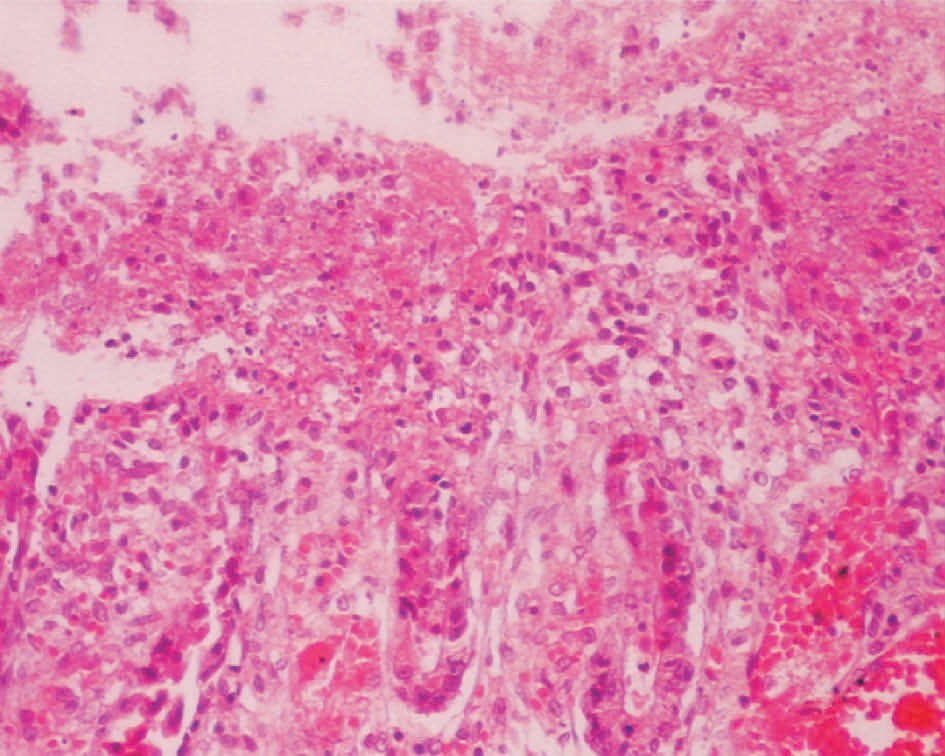
\includegraphics{./images/Image00057.jpg}
 \caption{结肠假膜性炎(HE染色,高倍)\\ {\small 肠黏膜上皮变性坏死,与渗出的纤维素及白细胞等混杂,形成假膜。黏膜充血水肿,炎细胞浸润}}
 \label{fig4-6}
  \end{figure} 



\begin{figure}[!htbp]
 \centering
 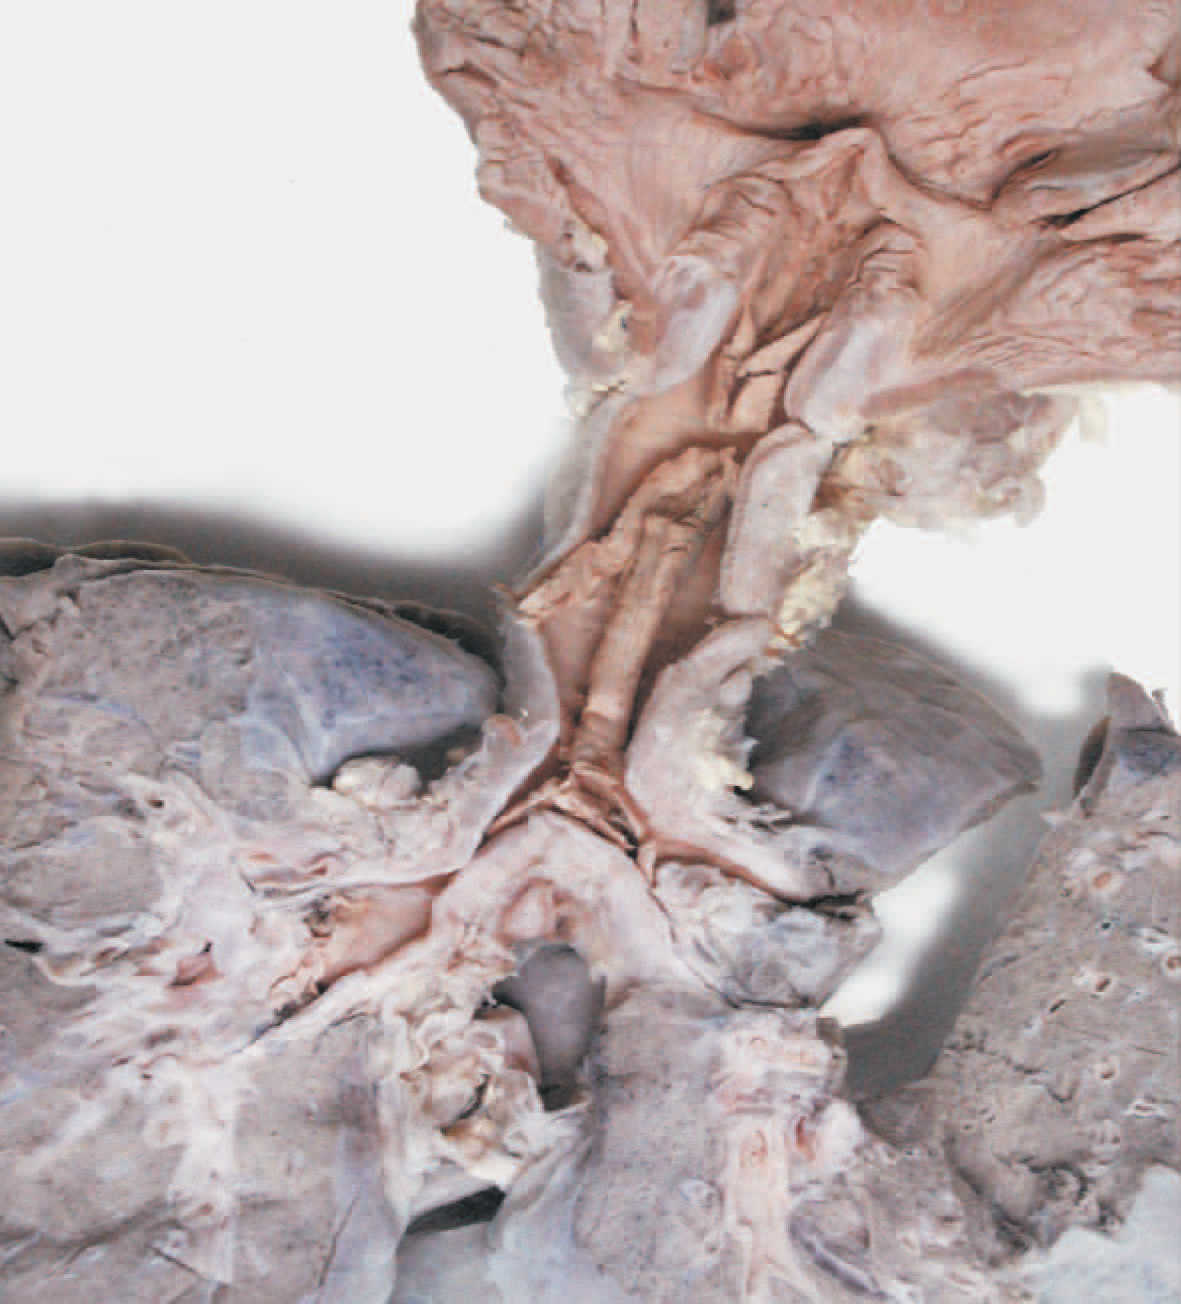
\includegraphics{./images/Image00058.jpg}
 \caption{白喉\\ {\small 气管及主支气管内可见剥脱的假膜}}
 \label{fig4-7}
  \end{figure} 



浆膜的纤维素性炎常见于胸膜腔和心包腔,如肺炎球菌引起的纤维素性胸膜炎,风湿及心肌梗死引发的纤维素性心外膜炎(图\ref{fig4-8}),心外膜的纤维素性渗出物由于心脏的不停搏动而呈绒毛状,又称``绒毛心''。

\begin{figure}[!htbp]
 \centering
 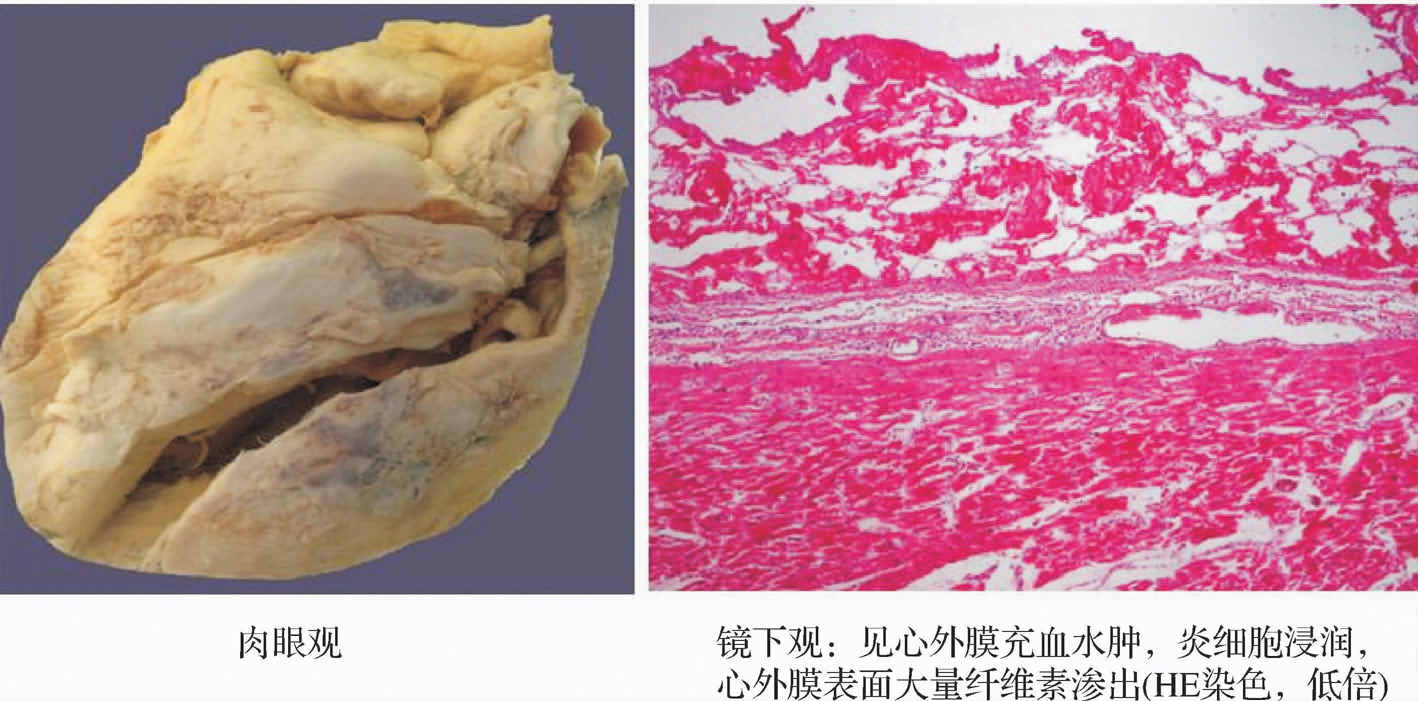
\includegraphics{./images/Image00059.jpg}
 \caption{纤维素性心外膜炎}
 \label{fig4-8}
  \end{figure} 

纤维素性渗出物一般可通过中性粒细胞释放的蛋白溶解酶溶解吸收,但如果炎症时渗出的纤维素过多或中性粒细胞释放的蛋白溶解酶不足(如白细胞缺乏症、中性粒细胞蛋白溶解酶缺陷病人),则渗出的纤维素不能全部被降解吸收,只能通过肉芽组织增生的方式发生机化,因此可造成器官、组织大量纤维结缔组织增生,功能受到严重影响。

{3. 化脓性炎}  化脓性炎(suppurative or purulent
inflammation)以大量中性粒细胞渗出为主,并伴有不同程度的组织坏死和脓液形成为特点。

化脓性炎多由葡萄球菌、链球菌、大肠埃希菌等化脓菌引起,也可由某些化学物质引起,如将松节油注入组织内引起的化脓。这种非细菌因素引起的化脓现象称为``无菌性化脓''。化脓性炎时,炎症灶中的细胞、组织在细菌和中性粒细胞释放的蛋白溶解酶的作用下发生液化坏死,加上血管的液体渗出,形成肉眼呈黄白色的浓稠液体,称为``脓液''(pus)。脓液中的中性粒细胞除极少数仍有吞噬能力外,大多数已发生变性和坏死,称为脓细胞。脓液中除含有脓细胞外,还含有大量的细菌、坏死组织碎片和少量浆液。视感染细菌种类的不同,脓液可呈不同的颜色、气味和黏稠度,借此特征常可大致判断感染细菌的种类。化脓性炎有以下三种主要的病理类型:

(1)表面化脓和积脓:表面化脓是指浆膜或黏膜的化脓性炎,且炎症仅限于浆膜或黏膜的浅层,脓液主要向黏膜或浆膜表面渗出,深部组织的炎症不明显,如化脓性尿道炎、化脓性支气管炎等。如果表面化脓渗出的脓液积聚在浆膜腔或空腔脏器内(如胆囊、输卵管等),则称为``积脓''(empyema)。

(2)脓肿(abscess):局限性化脓伴有脓腔形成的化脓性炎称为脓肿(图\ref{fig4-9}),常由金黄色葡萄球菌引起。金黄色葡萄球菌感染不仅使组织发生液化坏死,同时由于其血浆凝固酶的作用使渗出的纤维蛋白原转变为纤维素,使病变比较局限。早期脓肿边缘组织充血水肿、炎细胞浸润,以后肉芽组织逐渐增生,形成包绕脓腔的脓肿膜。脓肿膜具有限制病变扩散的作用,但过厚的脓肿膜也使脓液吸收困难,药物也不易进入,因此往往需要手术切开排脓或穿刺抽脓。脓液及坏死物清除干净后,由肉芽组织填补修复,最后形成结缔组织瘢痕。

\begin{figure}[!htbp]
 \centering
 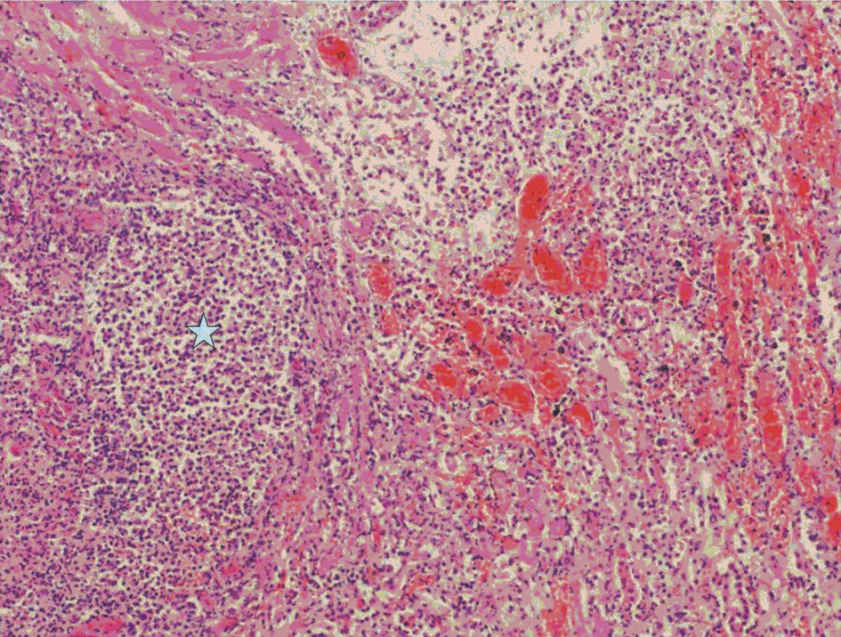
\includegraphics{./images/Image00060.jpg}
 \captionsetup{justification=centering}
 \caption{肾脓肿(HE染色,低倍)\\ {\small 肾组织充血水肿,大量中性粒细胞浸润。白星号示脓肿灶,局部肾组织完全坏死、液化,伴有大量脓细胞聚集}}
 \label{fig4-9}
  \end{figure} 



疖(furuncle)是毛囊、皮脂腺及其周围组织的脓肿。疖中心部分液化变软后,脓液便可破出。痈是多个疖的融合,在皮下脂肪和筋膜组织中形成许多相互的脓肿,必须及时切开排脓。

皮肤、黏膜浅部的脓肿可向表面破溃而形成较大的缺损,称为溃疡(ulcer)。深部组织的脓肿如向体表或自然管道穿破,可形成一端开口的盲管,称为窦道(sinus)。如果深部脓肿形成体表与有腔器官之间或两个有腔器官之间的有两个以上开口的病理性管道,则称为瘘管(fistula)。例如,肛门周围组织的脓肿可向皮肤穿破,形成窦道;也可以一端穿破皮肤,另一端穿入直肠肛管而形成两端连通的瘘管称为肛瘘(图\ref{fig4-10})。由于窦道、瘘管不断排出脓液,因此病变较难愈合。

\begin{figure}[!htbp]
 \centering
 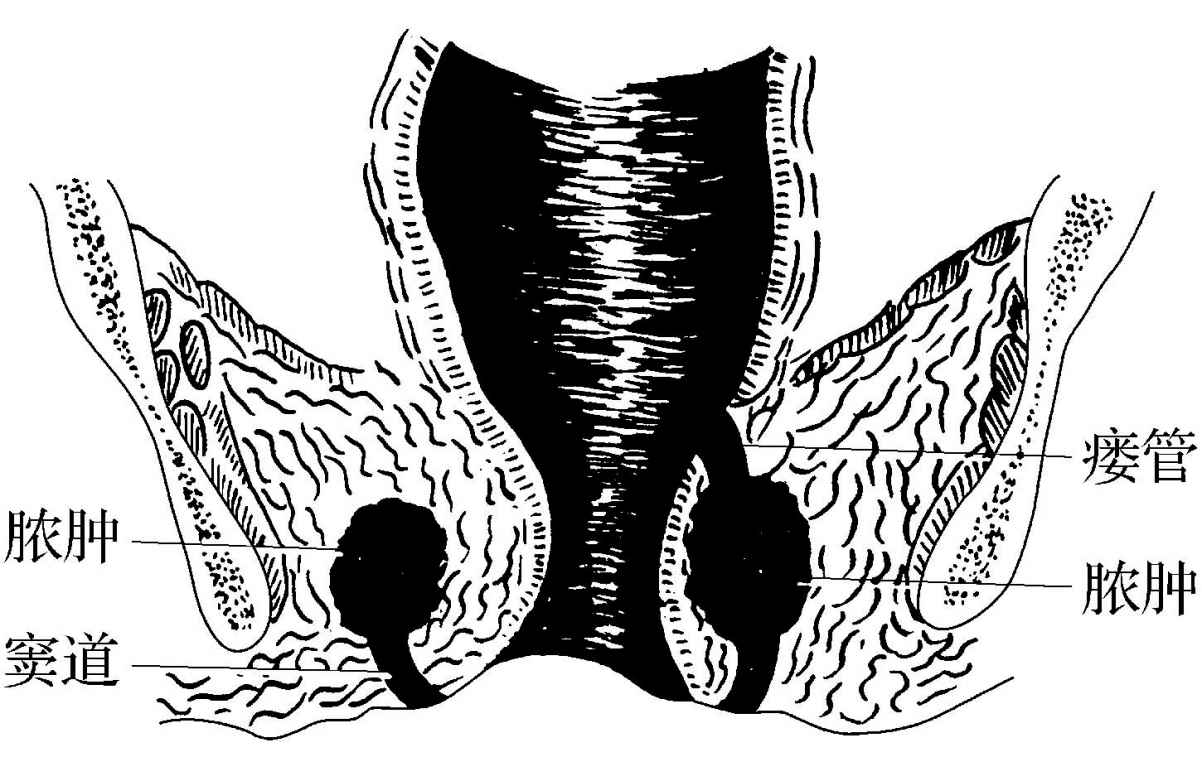
\includegraphics{./images/Image00061.jpg}
 \caption{肛门周围脓肿 \\ {\small 窦道、瘘管形成}}
 \label{fig4-10}
  \end{figure} 


\begin{framed}
{案例4-1}

{【病例摘要】}

患者,男,75岁,因颈部肿痛伴发热2周入院。患者2周前出现颈部皮肤肿胀、疼痛,范围逐渐扩大,疼痛加剧。体检:背部可见约5
cm×4.5
cm圆形皮肤隆起,暗红色,表面可见多个脓点,部分已破溃流脓,触痛明显,颈部可扪及多个肿大的淋巴结,有触痛。血常规:白细胞计数15.6×10{9}
/L,中性粒细胞87%。

{【问题】}

(1)该患者颈部病变是什么?

(2)该病变属于哪种类型的炎症?
\end{framed}

(3)蜂窝组织炎(phlegmonous
inflammation):又称蜂窝织炎,是指疏松结缔组织内的弥漫性化脓性炎,常见于皮肤、肌肉和阑尾。蜂窝组织炎主要由溶血性链球菌引起,链球菌分泌的透明质酸酶和链激酶可降解组织间质中的基质成分(透明质酸和纤维素等),因此细菌很容易通过组织间隙蔓延扩散。病变的组织高度水肿,与正常组织分界不清晰,大量中性粒细胞浸润,但组织液化坏死不明显(图\ref{fig4-11})。

\begin{figure}[!htbp]
 \centering
 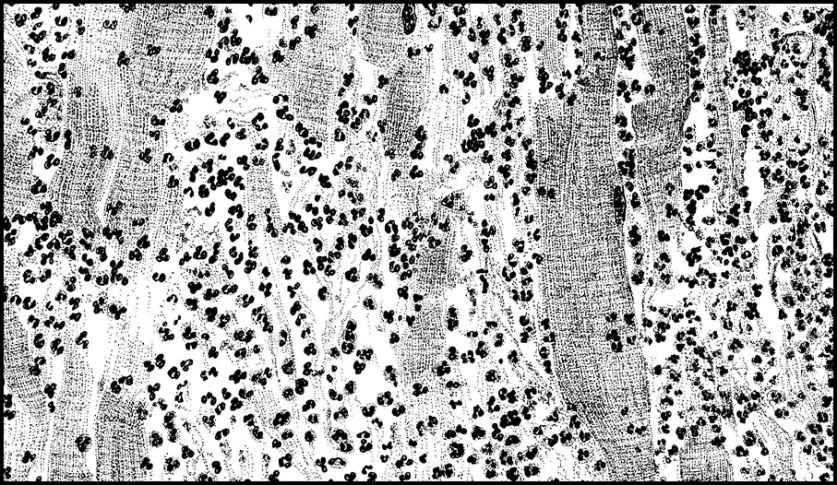
\includegraphics{./images/Image00062.jpg}
 \caption{横纹肌蜂窝组织炎 \\ {\small 组织水肿,肌纤维间大量中性粒细胞浸润,部分肌纤维变性坏死}}
 \label{fig4-11}
  \end{figure} 



{4. 出血性炎}  出血性炎(hemorrhagic
inflammation)并非独立的一种炎症类型。当炎症过程中血管壁损伤严重,通透性极度增高时,导致大量红细胞的漏出,即可称出血性炎。常见于肾综合征出血热、钩端螺旋体病和鼠疫等。

上述几种炎症类型可单独发生,也可几种同时并存,如浆液纤维素性炎、纤维素性化脓性炎等。一种类型的炎症也可以转变为另一种类型的炎症。

{(三)增生性炎}

大多数急性炎症局部的病变以变质和渗出为主,但也有少数急性炎症以增生性改变为主,这类炎症称为增生性炎(proliferative
inflammation)。例如,急性弥漫性增生性肾小球肾炎,病理变化主要为肾小球毛细血管内皮细胞和系膜细胞增生;早期伤寒的病理变化则表现为单核巨噬细胞增生为主。

\section{慢性炎症}

慢性炎症一般起病较缓,病程较长(数月至数年)。慢性炎症除了缓慢起病、逐渐出现临床症状以外,也可以由急性炎症的病程延长、病变发生变化转变而来。部分病人甚至发病后没有明显的临床症状,等到出现临床表现时已属疾病的晚期。约有25%的慢性硬化性肾小球肾炎病人,起病缓慢,无自觉症状,无肾炎病史,发现时已为晚期,可出现各种严重的并发症。慢性炎症局部的病变以增生为主,浸润的炎细胞主要为淋巴细胞、浆细胞及巨噬细胞,血管扩张充血、渗出、变质性改变常不明显。

慢性炎症发病机制十分复杂,其发生原因主要为:病原微生物长期存在、理化因子长期刺激和自身免疫反应;淋巴细胞、巨噬细胞持续激活以及各种细胞因子不断释放可能是慢性炎症发展的关键机制。

根据形态学特点,慢性炎症可分为非特异性慢性炎和慢性肉芽肿性炎两大类。

\subsection{非特异性慢性炎}

非特异性慢性炎病变主要表现为纤维母细胞、血管内皮细胞和组织细胞增生,伴有淋巴细胞、浆细胞和巨噬细胞等慢性炎细胞浸润,同时局部的被覆上皮、腺上皮和实质细胞也可增生。慢性炎症还可伴有肉芽组织的形成。这类炎症常见于有较大组织缺损的病变,此时肉芽组织在慢性脓肿、瘘管和慢性黏膜溃疡的吸收和分解上起重要作用。

长期慢性炎症使局部黏膜上皮、腺体及间质增生,形成带蒂、向表面突起的肉样肿块,称为炎性息肉(inflammatory
polyp),常见于鼻黏膜、肠黏膜及子宫颈黏膜(图\ref{fig4-12})。若炎性增生形成境界清楚的肿瘤样肿块,则称为炎性假瘤(inflammatory
pseudotumor),常发生于眼眶和肺,须与真性肿瘤鉴别。

\begin{figure}[!htbp]
 \centering
 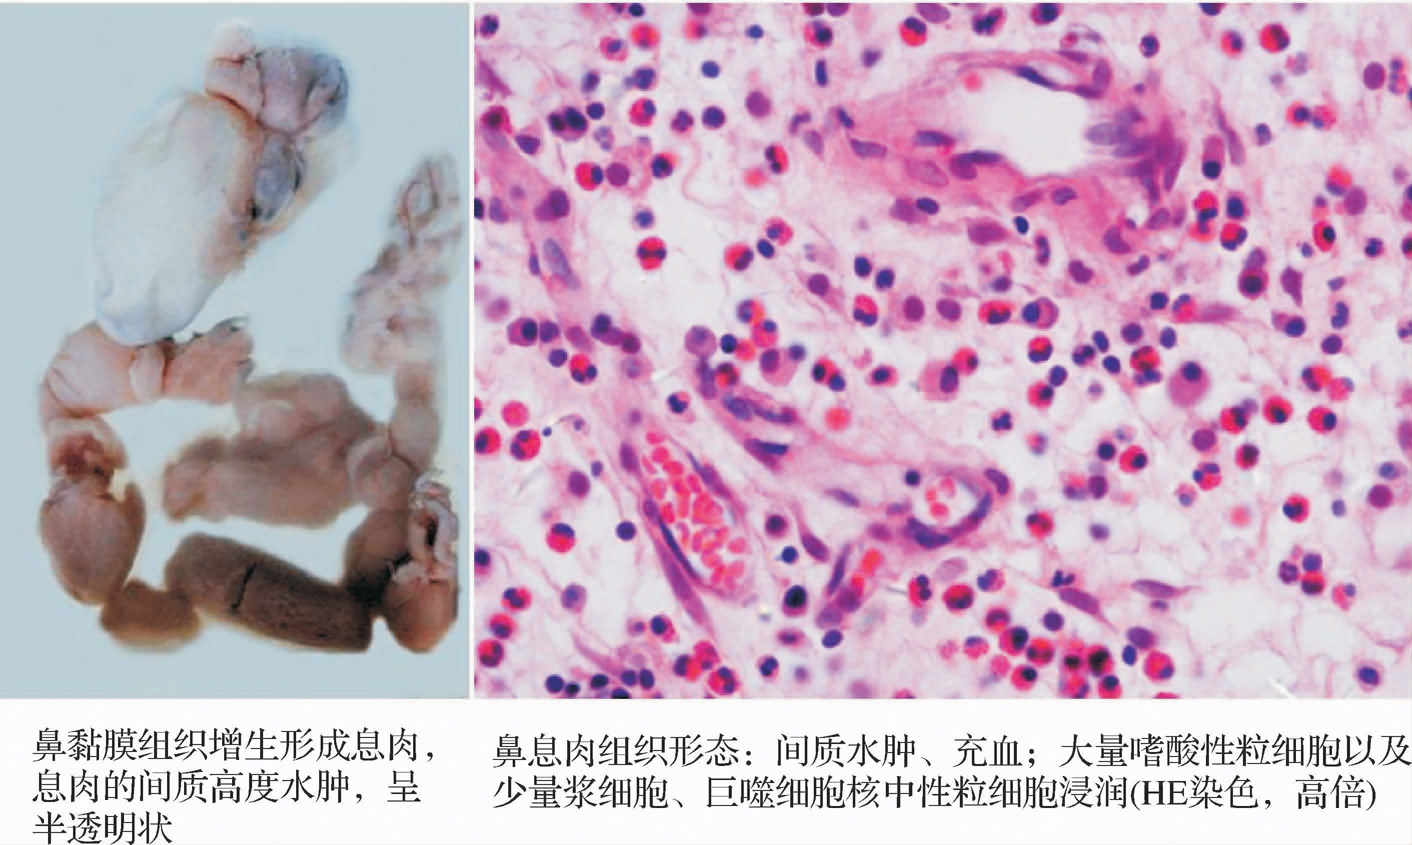
\includegraphics{./images/Image00063.jpg}
 \caption{慢性鼻炎}
 \label{fig4-12}
  \end{figure} 

\subsection{慢性肉芽肿性炎}

以单核巨噬细胞增生为主,形成结节状、境界清楚的增生性病灶称为肉芽肿(granuloma),以肉芽肿形成为特征的慢性炎症称为慢性肉芽肿性炎(chronic
granulomatous inflammtion)。肉芽肿的结节较小,一般直径为0.5~2
mm。根据致炎因子的不同,肉芽肿可分为感染性肉芽肿和异物性肉芽肿。感染性肉芽肿由生物病原体如结核杆菌、伤寒杆菌、麻风杆菌、梅毒螺旋体、真菌和寄生虫等引起,异物性肉芽肿多由手术缝线、木刺、粉尘、滑石粉等异物引起。此外,有些自身免疫性疾病也可引起肉芽肿形成(如风湿病、Wegener's肉芽肿)。

构成肉芽肿的基本成分为单核巨噬细胞,不同病因引起的肉芽肿形态不完全一致,根据典型肉芽肿的形态特征往往可以判断其病因。以结核杆菌引起的结核性肉芽肿(结核结节)为例(图\ref{fig4-13}),其形态结构由内向外依次为:

{1. 干酪样坏死}
 有的结核结节中心为干酪样坏死,内含坏死的组织细胞、白细胞和结核杆菌,组织坏死彻底,镜下仅见一些无定形的颗粒状物质,这可能是细胞免疫介导免疫反应的结果。

{2. 类上皮细胞}
 类上皮细胞是结核性肉芽肿中增生的单核巨噬细胞的主要类型。在巨噬细胞趋化因子(MCF)、巨噬细胞游走抑制因子(MIF)和巨噬细胞活化因子(MAF)等细胞因子的刺激下,巨噬细胞在炎症局部大量增生并活化,表现为细胞体积增大,细胞之间境界不清,细胞浆更加丰富,细胞器增多(特别是内浆网、溶酶体增多),胞核呈圆形或椭圆形,染色质少。因这种细胞形态与上皮细胞相似,故称为类上皮细胞或上皮样细胞(epithelioid
cell)。

有人认为,活化的巨噬细胞杀菌能力大大加强的原因主要不是吞噬能力的增强(由于细胞表面Fc受体和C{3b}
受体的减少,其吞噬能力甚至是降低的),而是由于杀菌物质的细胞外分泌作用而杀伤细胞周围的细菌,同时在宿主健康组织与细菌之间形成一条隔离带。

{3. 多核巨细胞}  结核性肉芽肿的类上皮细胞之间还可见到一种体积大(40~50
μm)、胞浆丰富、多核(数十个核)的巨细胞。多核巨细胞是由类上皮细胞相互融合而成或细胞核有丝分裂而胞浆不分裂形成的。结核杆菌等感染时形成的多核巨细胞称为朗汉斯巨细胞(Langhans
giant
cell),其细胞核的排列很有特点,呈马蹄形或花环状排列在细胞的周边部。由异物(手术缝线、木刺等)引起的肉芽肿中也可见到多核巨细胞,但其细胞核往往排列杂乱无章,不像郎汉斯巨细胞那样有规律,此种细胞称为异物巨细胞(foreign
body-type giant cell)。多核巨细胞的功能与类上皮细胞的功能相似。

{4. 淋巴细胞}
 肉芽肿的周边部可见大量淋巴细胞浸润,说明结核肉芽肿的形成与细胞免疫关系密切。

{5. 纤维母细胞}
 结核肉芽肿的周边部还可见到纤维母细胞及其产生的胶原纤维。随着病原体的杀灭及病变的发展,肉芽肿最终将由纤维母细胞产生的胶原纤维取代而形成纤维化的细小瘢痕。

\begin{figure}[!htbp]
 \centering
 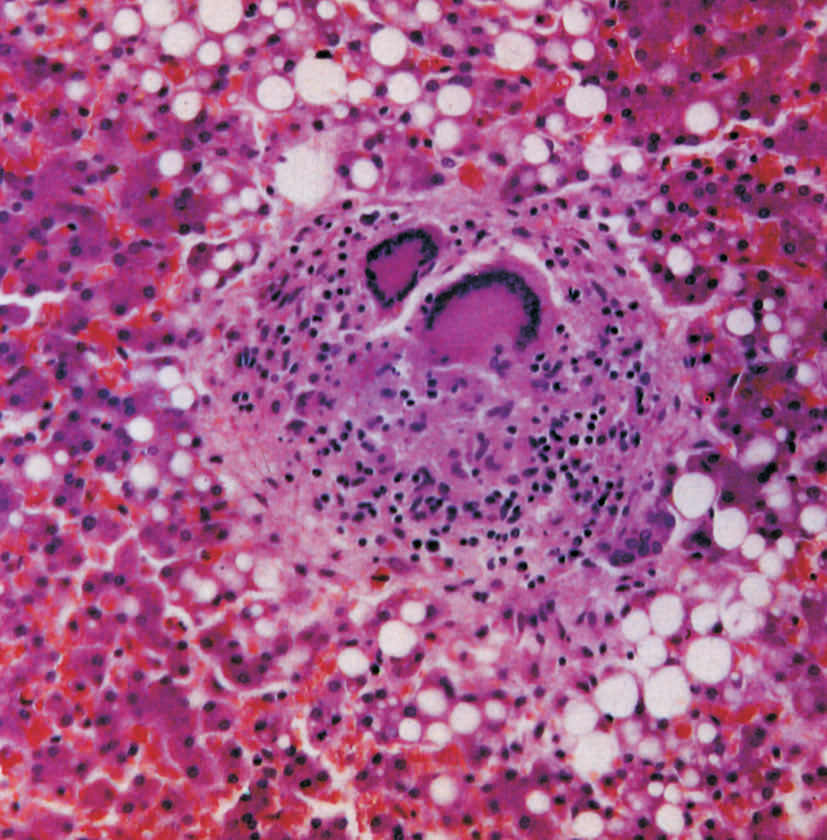
\includegraphics{./images/Image00064.jpg}
 \caption{肝结核结节(HE染色,高倍)\\ {\small 由类上皮细胞、朗汉斯巨细胞、淋巴细胞、纤维母细胞等组成}}
 \label{fig4-13}
  \end{figure} 



{知识链接}

Langhans细胞和Langerhans细胞,是两种完全不同的细胞,却因为拼写类似,时常被混淆,甚至就连国际著名的《柳叶刀》杂志(Lancet)也难免疏忽。Langhans细胞为结核性肉芽肿的特异性多核巨细胞,由Theodor
Langhans(1839---1915)发现。Langerhans细胞为表皮间隙的树突状细胞,可发生Langerhans组织细胞增多症,由Paul
Langerhans(1847---1888)发现。有趣的是,这两位德国病理学家不仅姓氏相似,其研究结果在同一年(1868年)的同一本杂志(Virchow's
Archives)上发表,最后两位病理学家居然死于同一种疾病(结核病)。[Pritchard
J,Foley P,Wong H. Langerhans and Langhans:what's misleading in a
name?Lancet,2003 362(9387):922]

\section{炎症的临床表现和结局}

\subsection{炎症的局部表现与全身反应}

{(一)炎症的局部表现}

炎症的局部表现主要为红、肿、热、痛和功能障碍。炎症局部血管扩张、血流加快及代谢增强使炎症局部出现发红、发热现象。炎性水肿、炎细胞浸润(包括渗出和增生)可使炎症局部出现肿胀。致痛性炎症介质的直接作用和炎症局部的肿胀压迫神经末梢可引起疼痛。炎症灶中实质细胞的变性坏死和代谢障碍、炎性渗出时的机械性阻塞和压迫、疼痛性保护性反射引起的活动受限等都可能导致组织和器官的功能障碍。

{(二)炎症的全身反应}

炎症引起的全身反应主要有发热、外周血白细胞计数增高,有时还可见全身单核巨噬细胞系统的增生。

{1. 发热}
 发热在感染性炎症中十分常见,不同的病原体感染及感染的类型不同,发热的热型也不相同,如典型的伤寒病常表现为持续39~40℃达数日或数周的``稽留热'',而结核杆菌感染表现出的发热常为午后低热。引起发热的原因是内源性和外源性致热原的作用,外源性致热原是通过内源性致热原的作用而间接起致热作用的。细菌代谢产物尤其内毒素是常见的外源性致热原,而细胞因子如IL-2、TNF以及前列腺素是常见的内源性致热原。适当增高的体温使机体的代谢加快,白细胞的吞噬作用和抗体的生成都会增强,有利于炎症的康复。

{2. 外周血白细胞计数增高}
 特别是感染性炎症,有时白细胞计数可高达4×10{10}
个/L。外周血白细胞增多主要是骨髓加速释放和在集落刺激因子(colony
stimulating
factor,CSF)的刺激作用下,骨髓造血干细胞增殖所致。白细胞的增多具有重要的防御意义,但在某些炎症如病毒性感染、伤寒、严重感染,以及机体抵抗力极度降低的情况下,外周血白细胞计数可无明显增高,甚至降低,其预后较差。

{3. 单核巨噬细胞系统增生}
 有些炎症(如伤寒等),因为细菌或毒素进入血液,可刺激单核巨噬细胞系统增生,导致肝、脾、淋巴结肿大。

\subsection{炎症的结局}

{(一)痊愈}

通过机体的抗损伤反应和及时的治疗,大多数炎症可以痊愈。当坏死面积较小时,坏死组织在酶解作用下可以溶解吸收,通过完全性再生而痊愈。当炎症局部坏死范围较大时,只能通过机化、纤维包裹、钙化以及分离排出等方式痊愈,局部组织不能恢复原来的结构和功能,称为不完全痊愈。渗出性炎的液体成分在炎症恢复过程中常能完全吸收,但当纤维素渗出过多、中性粒细胞释放的蛋白溶解酶不足时,可发生机化,导致纤维结缔组织增生。慢性肉芽肿性炎恢复时,肉芽肿最终转变为纤维化的小结节,因为体积微小,一般不造成明显不良后果。但发生在特殊部位(如心脏)并反复发作的病变,由于纤维结缔组织逐渐增多,也会造成不良后果。慢性炎症由于实质细胞、间质细胞及结缔组织的大量增生,组织结构发生改变,因而即使炎症痊愈也多影响到器官的功能。

{(二)迁延不愈}

迁延不愈即急性炎症慢性化。急性炎症治疗不彻底或机体抵抗力时高时低,则致炎因子不能在短期内消除,炎症过程可迁延不愈,转化为慢性炎症。临床表现为病情时轻时重,常有慢性炎症急性发作。

{(三)扩散}

细菌等感染造成的炎症,当机体抵抗力低下,或病原体毒力强、数量多时,病原微生物可不断繁殖,向周围组织蔓延,或通过淋巴管、血管向全身扩散。

{1. 局部蔓延}
 病原微生物沿组织间隙或器官的自然管道向周围组织扩散,如肾结核可沿泌尿道下行扩散,引起输尿管和膀胱结核。

{2. 淋巴道扩散}
 病原体进入淋巴管,引起淋巴管和所属回流淋巴结的炎症,如上肢感染引起腋窝淋巴结肿大,下肢感染引起腹股沟淋巴结肿大等。淋巴结的反应可限制病原体的进一步扩散,但感染严重时,病原体也可通过淋巴液入血。

{3. 血道扩散}
 炎症灶中的病原微生物或其毒性产物可进入血液,引起菌血症、毒血症、败血症和脓毒败血症。

(1)菌血症(bacteremia):细菌由局部病灶入血,全身无中毒症状,但血液中可检测到细菌,称为菌血症。菌血症常发生在炎症的早期阶段,例如大叶性肺炎和流行性脑脊髓膜炎,肝、脾和骨髓的吞噬细胞可以清除细菌。

(2)毒血症(toxemia):细菌的毒性产物或毒素被吸收入血称为毒血症。例如白喉杆菌一般不进入血液,而是释放大量白喉毒素进入血液,出现全身中毒症状,同时伴有心肌细胞的变性或坏死,严重时出现中毒性休克。

(3)败血症(septicemia):毒力较强的细菌由局部病灶入血后,不仅没有被清除,而且还大量繁殖并产生毒素。此时不仅在血液可检测到细菌,更可引起高热、皮疹、肝脾肿大及全身淋巴结肿大等全身中毒表现和多系统多脏器的病理改变称为败血症。

(4)脓毒败血症(pyemia):如果引起败血症的细菌是金黄色葡萄球菌等化脓菌,则临床上除了有败血症的表现以外,细菌栓子还可栓塞于毛细血管,引起肝、肾等全身多脏器散在均匀分布的多发性小脓肿形成,此时称为脓毒败血症。

\begin{framed}
{案例4-2}

{【病例摘要】}

患儿,男,6岁,因发热、头痛、咽痛3天入院。患儿既往未按时接种百白破三联疫苗。体检:扁桃体中度红肿,其上可见乳白色或灰白色大片假膜,范围不超出扁桃体。入院后诊断为白喉,足量抗生素和对症治疗。入院后第2天突然出现呼吸困难、面部发绀,急行气管切开,纤维支气管镜从右主支气管中取出片状假膜状物,症状缓解。当晚患儿出现面色青紫,四肢厥冷、脉搏加快而弱、血压下降,呼吸急促,肺部大量湿啰音,咳粉红色泡沫样痰,心音低钝,抢救无效死亡。

{【问题】}

(1)该患儿支气管黏膜上的假膜,主要组成成分是什么?

(2)试分析抗生素疗效不佳和患儿死亡的原因。
\end{framed}

\section*{复习与思考}

{一、名词解释}

变质 渗出 增生 趋化作用 炎性息肉 假膜性炎 炎细胞浸润 化脓性炎 溃疡 炎症介质 炎性假瘤 脓肿 脓毒败血症 蜂窝织炎 窦道 瘘管 慢性肉芽肿性炎 绒毛心

{二、问答题}

1. 试述炎症的概念和炎症对机体的作用。

2. 举例说明变质、渗出、增生三者在炎症中的相互关系。

3. 举例说明常见的变质性炎、渗出性炎和增生性炎各自的特点。

4. 试述液体渗出的过程、机制及意义。

5. 试述白细胞渗出的过程、机制和意义。

6. 比较脓肿和蜂窝组织炎之间的异同。

7. 比较急性炎症和慢性炎症在组织病理学上的区别。

8. 何谓慢性肉芽肿性炎?常由哪些原因引起?其基本特征是什么?

9. 试述炎症的结局。

10. 试述炎症血道扩散的不同类型。

{三、临床病例分析}

患儿,男,12岁,因发热、腿痛半个月入院。于入院前15天开始感右腿肿胀疼痛,次日即出现发热、食欲减退、精神不佳。

体格检查:体温39.1℃,脉搏107次/分,呼吸36次/分,血压108/74
mmHg(14.4/9.9 kPa)。

右大腿有一肿块,局部发红、发热,并有压痛。白细胞:10.5×10{9}
/L,中性粒细胞:92%,淋巴细胞:7%,单核细胞:1%。B超检查发现肝、肺、肾及脑部均有多个肿块,其中脑部肿块约有5
cm×3 cm×2
cm。入院后切开右大腿肿块,排出大量脓液。入院后第五天,病人感到剧烈头痛、呕吐、烦躁不安,经抢救无效,出现呼吸心跳停止而死亡。

讨论题:

1. 患儿患的是什么疾病?并写出诊断依据。

2. 试说明病变的发生发展过程。

3. 本例患儿的主要死亡原因是什么?




